%%%%%%%%%%%%%%%%%%%%%%%%%%%%%
%    PAPER for MA 952/672
%    Tony Zhang
%%%%%%%%%%%%%%%%%%%%%%%%%%%%%

\documentclass[10pt]{article}

\usepackage{tony}

% for drawing figures and stuff
\usepackage{tikz}
\usetikzlibrary{matrix,chains,positioning,decorations.pathreplacing,arrows}

% new math operator
\DeclareMathOperator{\softmax}{softmax}

\title{Voice Classification by Neural Networks}
\author{
	\href{mailto:txz@mit.edu}{Tony Zhang},
	\href{mailto:jtsui@hotchkiss.org}{James Tsui},
	\href{mailto:mbahrani@hotchkiss.org}{Maryam Bahrani}
}

\begin{document}
\maketitle

\begin{abstract}
% TODO
% neural net to classify voice gender (age?)
% 

In this paper, we describe a machine learning schema for voice classification by sex. We collected %XXXXX
voice samples that we used to train an artificial neural net with a single hidden layer using stochastic gradient descent. After experimenting to determine the optimal training parameters (number of iterations, etc.), using %%10-fold cross-validation with ROC AUC as our metric to evaluate our model.
With % certain settings
we were able to produce a model that performs %stats
\end{abstract}

\section{Introduction}

% introduce things
% theory background

Though still a relatively new field, machine learning, the study of algorithms that can ``learn" dynamically, holds much potential.
Already, machine learning algorithms are finding great use in everything from identification of Higgs Boson decay events in high-energy particle collisions to recommendation systems on such sites as Facebook, YouTube, and Netflix.
% blah blah blah

A curious development in macine learning was the \emph{neural network} (or informally, a neural net), a biologically inspired machine learning model.
Indeed, we see how the nodes in \cref{fig:neuralnet} resemble neurons sending information to other neurons.
We shall soon offer a mathematically rigorous definition of the neural network.

The goal of a neural network is to classify \emph{instances} described by \emph{feature vectors}; that is, given some data about an instance (``features", e.g. the batting average of a particular baseball player, the temperature that particular day), we would like to place the instance into one of a number of \emph{classes} (e.g. this player's next swing will/will not be a strike).
In particular, the neural network will be a function taking input data and outputting some numbers that can be interpreted as the probability that this instance is in a particular class.\footnote{To be nitpicky, we should only say that these numbers are simply indices for the model's confidence that the instance is in some class.}

Let's make that concrete.
For our baseball example, suppose we'd like to predict whether Lauren the baseball player (batting average 0.315) will hit the ball on her next swing.
The current temperature at the stadium is 21.6 degrees Celsius.
So we give the neural net the feature vector $(0.315, 21.6)$.
The neural net then outputs us $(0.21, 0.79)$---a strike with ``probability" 0.21 and a non-strike with ``probability" 0.79.

% picture of neural net
\begin{figure}[htbp]
\centering
% this code is derived from code in the following stackexchange answer
% http://tex.stackexchange.com/a/132471
\begin{tikzpicture}[
plain/.style={
    draw=none,
    fill=none,
},
    net/.style={
        matrix of nodes,
        nodes={
            draw,
            circle,
            inner sep=10pt
        },
        nodes in empty cells,
        column sep=2cm,
        row sep=-9pt
    },
    >=latex
    ]
\matrix[net] (mat)
{
    |[plain]| \parbox{1.3cm}{\centering Input\\layer} & |[plain]| \parbox{1.3cm}{\centering Hidden\\layer} & |[plain]| \parbox{1.3cm}{\centering Output\\layer} \\
        & |[plain]| \\
        |[plain]| & \\
        & |[plain]| \\
        |[plain]| & |[plain]| \\
        & & \\
        |[plain]| & |[plain]| \\
        & |[plain]| \\
        |[plain]| & \\
        & |[plain]| \\
};
\foreach \ai [count=\mi ]in {2,4,...,8}
\draw[<-] (mat-\ai-1) -- node[above] {Input \mi} +(-2cm,0);
\foreach \ai in {2,4,...,10}
{\foreach \aii in {3,6}
    \draw[->] (mat-\ai-1) -- (mat-\aii-2);
}

\draw[<-] (mat-10-1) -- node[above] {Bias} +(-2cm,0);

\foreach \ai in {3,6,9}
\draw[->] (mat-\ai-2) -- (mat-6-3);
\draw[->] (mat-6-3) -- node[above] {Ouput} +(2cm,0);

\draw[<-] (mat-9-2) -- node[above] {Bias} +(-2cm,0);
\end{tikzpicture}

\caption{A simple neural network.}
\label{fig:neuralnet}
\end{figure}

% describe our project

\subsection{Neural Net Theory}

What exactly is a neural net, and how does it make these predictions?
Each neural net takes some input and sends it through a set of \emph{neurons}, each carrying a value, organized into \emph{layers}.
(\cref{fig:neuralnet} displays 3 layers, but a neural net can have arbitrarily many layers, with arbitrarily many neurons in each.)
The value of each neuron is either predetermined (as are the ``bias" neurons in \cref{fig:neuralnet}, whose values are fixed at 1, or the input neurons, whose values are just the individual components of the feature vectors---one input neuron could contain a baseball player's batting average, for example) or computed from the values of neurons in the previous layer.
We read off the output of the neural net in the final layer, each of whose neurons will give us values in $(0, 1)$. There is one neuron per class, each representing the level of certainty the model has that our instance belongs to the respective class of the neuron.

For our purposes, each neuron $z$ (except for the bias neuron) in a \emph{hidden layer} (layer that isn't the first or last) depends on the neurons $x_i$ in the previous layer as follows:
\beq
\label{eq:hiddenlayer}
z = \sigma\left(\sum_i \alpha_i x_i \right)
\eeq
where $\sigma(t) = (1 + \exp(-t))^{-1}$ is the logistic function and the $\alpha_i$ are some known constants (imagine these as unique ``weights" attached to each arrow between neurons in \cref{fig:neuralnet}).
We shall see later where the values of $\alpha$ come from.

The values of the neurons $y_k$ ($k = 1, \dots, K$) in the output layer, however, are defined as follows:
\beq
y_k = \softmax_k(n_1, n_2, \dots, n_K) = \frac{\exp(n_k)}{\sum_j \exp(n_j)}
\eeq
where each $n_k$ is a ``proto-value" associated with neuron $y_k$ with value
\beq
\label{eq:netvalue}
n_k = \sum_i \beta_i x_i
\eeq
where the $\beta_i$ are known constants (like the $\alpha_i$ from a little before) and the $x_i$ are the neurons in the penultimate layer.

In general, with the exception of the input neurons and the bias neurons, each neuron's value is simply produced by applying some nonlinear function (e.g. $\sigma, \softmax$) to a linear combination of the values of the neurons in the previous layer.
The weights on the linear combination are predetermined.
Clearly, ``training" a neural net reduces to determining the correct weights for the situation.

\subsection{Gradient Descent}

% insert stuff about gradient descent!
Formally, we can rephrase our problem as follows: Given a set of $K$ instances $(x_k, y_k)$ and a family of functions $f(\vec{w})$,\footnote{Note that $f$ itself is a function $f:W\to X$, where $W$ is the space of all possible combinations of weights and $X$ is the space of functions from inputs---our features---to outputs---our predictions. Thus, $\vec{w}$ is a vector whose components are the parameters that determine our model.} find the parameters that minimize the inaccuracy of the estimates $f(\vec{w})(x_k)$ of $y_k$.
In particular, we are minimizing some \emph{objective function} dependent on both the instances and the parameters that quantifies that inaccuracy.
For our purposes, we will minimize mean-square error, defined as
\beq
\label{eq:meansqerror}
E(\vec{w}) = \sum_k E_k(\vec{w}) = \sum_k (y_k - f(\vec{w})(x_k))^2
\eeq

In practice, there will be numerous parameters (each $\alpha$ and $\beta$ in \cref{eq:hiddenlayer,eq:netvalue} is a component of $\vec{w}$), so finding a global minimum will be challenging: setting the derivatives of $E$ to 0 and solving the resulting nonlinear equations (our $f$ will involve the nonlinear logistic $\sigma$ and softmax functions) is unfeasible.
Instead, we will employ a technique known as gradient descent.

The basic idea is simple.
Suppose we are looking for low points in some terrain.
We pick an arbitrary location to begin.
Then, we walk downhill (in the direction of steepest descent) a certain distance.
We stop, then check which way will take us down the steepest path from our new location.
We walk downhill in that direction a certain distance again, then repeat the process.
Clearly, gradient descent will \emph{not} necessarily find the global minimum, but rather a local one.

We formalize this idea as follows.
Given an objective function $E$, we start with some arbitrary set of weights $\vec{w}_0$.
To find a better estimate for $\vec{w}$, we iteratively go ``downhill" from $\vec{w}_{n-1}$ to $\vec{w}_{n}$, computing
\beq
\label{eq:graddescent}
\vec{w}_n = \vec{w}_{n-1} - \eta\vec{\nabla} E(\vec{w}_{n-1})
\eeq
where $\eta > 0$ is some fixed step size (the ``certain distance" in our hill analogy).
The gradient $\vec{\nabla} E$ represents the direction of steepest ascent of the function $E$.
Gradient descent is extremely useful for our purposes because for the $E$ we are using, as the resulting derivatives $\frac{\partial E}{\partial w}$ are relatively simple to determine.

Still, since our objective function sums over all $K$ our instances $(x_k, y_k)$ (see \cref{eq:meansqerror}), gradient descent quickly becomes computationally expensive for us as we try to compute $O(K)$ partial derivatives.
Is there a more efficient alternative?

\subsubsection{Stochastic Gradient Descent}

Returning to \cref{eq:meansqerror}, we find that our error can be expressed as the sum of the errors on each individual instance.
Instead of minimizing $E = \sum_k E_k$, we can try to minimize an \emph{individual} $E_k$ (imagine replacing $E$ with $E_k$ in \cref{eq:graddescent}).
In the long run, we have reason to expect this procedure also minimizes $E$.

% TODO continue

\subsection{Receiver Operating Characteristic (ROC)}

Though our goal will ultimately be to find the feature vectors and training procedure that will result in the \emph{best} model, we have not yet introduced any metric for evaluating our models.
We shall now do just that.

For a binary classification model, where each instance is classified as in or not in some particular group (e.g. the next swing will/won't be a strike), we define the \emph{true positive rate} as the fraction of the instances in the group that are classified as such by the model.
Similarly, the \emph{false positive rate} is the fraction of the instances \emph{not} in the group that are still classified as in the group by the model.
A disease test with true and false positive rates 99\% and 5\% will successfully detect disease 99\% of the time.
On the other hand, it will detect disease in 5\% of all uninfected individuals.
Let us say that this disease test falls at $(0.05, 0.99)$ in \emph{receiver operating characteristic (ROC) space}, a coordinate plane where false and true positive rates are plotted on the $x$ and $y$ axes, respectively.

Recall that our neural net has \emph{continuous output}---rather than tell us whether some instance is in a class or not, it gives us a number in $(0, 1)$ that serves as an index of its confidence that the instance is in the class.
To convert this continuous output into a binary prediction (in/not in the class), we can set a threshold for this index.
Those instances for which the neural net gives us a result above the threshold are considered predicted to be in the class, and \emph{vice versa}.

As we vary the threshold, the neural net's position in ROC space will vary.
In particular, as we vary threshold from 0 to 1, the neural net will trace out a curve in ROC space (see \cref{fig:rocexample}), which we will call the model's \emph{ROC curve}.
Note that a random classifier, with no distinguishing power between positive and negative instances, would have an ROC curve coinciding with the line $y = x$, as we expect equal true and false positive rates from this classifier.
On the other hand, a model whose ROC curve lies above this line would tend to give higher ``scores" (the continuous output) to positive instances than to negative ones.
Thus, we would like our model's ROC curve to lie as far above the line $y = x$ as possible.

This intuition suggests that a good metric for evaluating our models could be the area under the ROC curve.
Indeed, \emph{Area Under Curve} (AUC) is a common metric for binary classification.
Its value can range from 0 to 1, though in practice, our values will lie in $(0.5, 1)$.
A value of 0.5 corresponds to a model no better than a random classifier, while a value of 1 corresponds to a model that perfectly distinguishes between positive and negative instances.

\begin{figure}
\centering
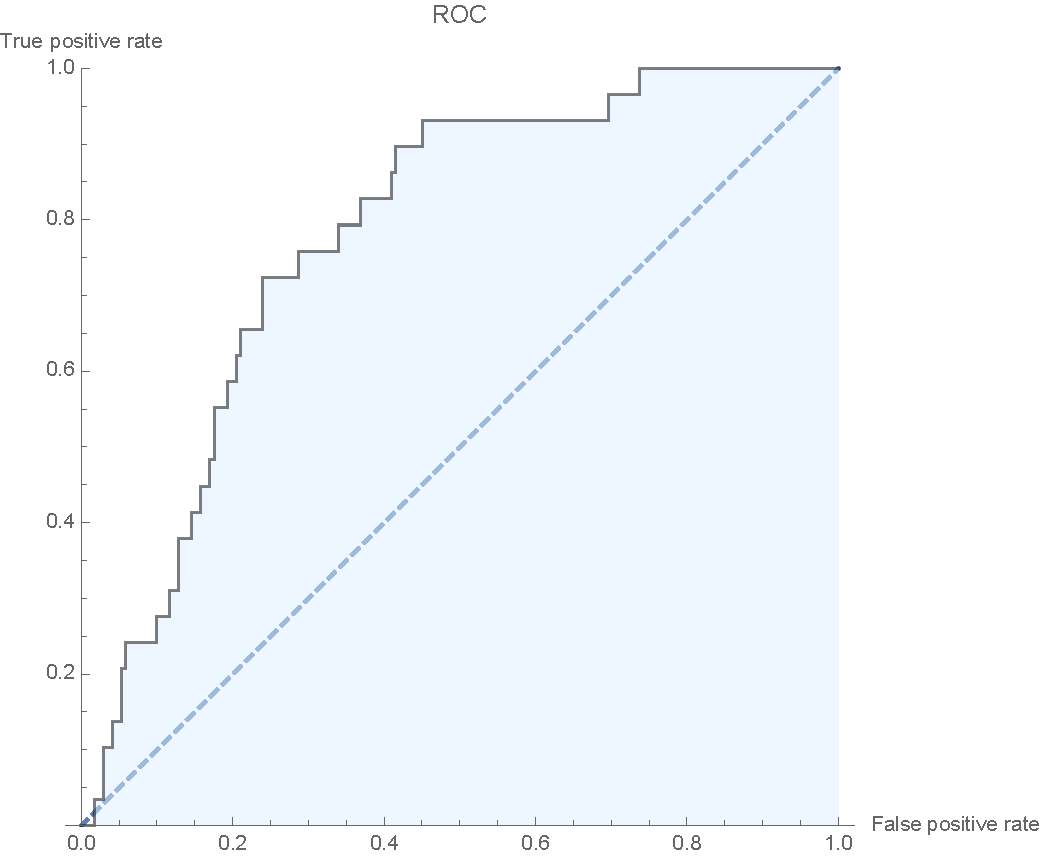
\includegraphics[width=\textwidth]{aux/rocexample.pdf}
\caption{An example ROC curve, with AUC $\approx 0.7804$. The dashed line shows $y = x$.}
\label{fig:rocexample}
\end{figure}

\subsection{Cross Validation}

% why do we want it? +overfitting
% training/test data


\subsection{Fourier Analysis}

% TODO
% discrete fourier analysis


\section{Methodology}

% TODO
% number of instances
% feature vectors (and which ultimately chosen): Tony
% structure of neural net
% gradient descent

% We collected XXXXXXXX voice samples, of which YYYYY were male and ZZZZZ were female.

Subjects were selected based on availability, with a majority of participants being students of the Hotchkiss School.
Voice recordings were collected from a total of $n = 63$ subjects (27 male and 36 female). 

Subject voice data was obtained in the form of 22050 Hz \texttt{.aiff} files, recorded using the microphone of an iPhone.
Subjects were instructed to speak until they were told to stop, and an approximately 10 second recording of their speech was made.
The sex and age of the subjects were recorded.
Although recorded, subject’s age is likely to be insignificant due to the stabilization of most voices post-puberty. Some subjects were given novels and other reading material to read from, as they were uncomfortable with speaking without directives.
This data was collected in relatively silent locations, thus minimizing background or stray noises. 

All data processing and analysis was completed in Wolfram Mathematica.
The voice samples were imported and processed using Fourier analysis.
We experimented with multiple schemata for feature extraction, before ultimately settling on the best for our purposes.
Each voice sample was broken into 0.5 second fragments (any trailing data at the end of the sound sample was discarded).
We took the norms of the discrete Fourier transform (DFT) of each fragment and added them together (i.e. if fragments $1, 2, \dots, n$ have DFTs $\hat{f_1},\hat{f_2}, \dots, \hat{f_n}$, we find $g = \sum_k |\hat{f_k}|$). The resulting function $g$ was normalized as in \[\bar{g} = \frac{g}{\sum\limits_m g(m)}\] where we sum over all $m$ in the (finite) domain of $g$.\footnote{As we are working with half-second fragments of 22050 Hz sound files, this domain is actually $\frac{\ZZ}{11025\ZZ}$.} Each voice file was analyzed thus, and a series of features were generated for each; these features constituted a profile of each subject's voice.





\section{Results}

% ROC AUC scores and such

\end{document}
